\chapter[Background and Related Works]{Background}

\section{Background Materials}
\subsection{Ahead-of-time (AOT) Compilation}
In Java programming, code compilation can occur either at build time or runtime. Ahead-of-Time (AOT) compilation involves translating the entire source code into machine code before execution, resulting in a fully compiled binary that is immediately executable \cite{Wade2017}. In contrast, Just-In-Time (JIT) Compilation defers the translation until runtime, dynamically converting Java bytecodes into machine code within the Java Virtual Machine (JVM) and optimizing frequently executed code paths to enhance performance \cite{Wade2017}. AOT compilation generally requires longer build times but offers rapid startup and predictable performance, making it suitable for applications where quick initialization is critical. JIT compilation, while benefiting from shorter build times, incurs longer startup periods but allows for more complex optimizations based on runtime data.

JIT compilation enables advanced techniques such as speculative optimizations, which involve making assumptions about a program’s behavior to apply performance-enhancing transformations based on runtime profiling. Although these optimizations can significantly improve performance by optimizing frequently executed code paths, incorrect assumptions may necessitate deoptimizations, which revert the code to a less optimized but more reliable version \cite{Duboscq2013Inproceedings}. This can complicate the intermediate representation (IR) of the code by adding additional nodes and edges to accommodate these transformations \cite{Duboscq2013Inproceedings}. In this project, the emphasis will be on AOT compilation, where speculative optimizations are excluded \cite{Wimmer2019}, resulting in a simpler IR without the need for deoptimization.

\subsection{GraalVM Compiler Optimizations}

In GraalVM, the compilation process is divided into two main phases. The first phase, involving the Graal Intermediate Representation (Graal IR), handles most of the high-level optimizations. This phase is further organized into three tiers: high-tier for high-level optimizations, mid-tier for memory-focused enhancements, and low-tier for low-level IR (LIR) conversion \cite{Graal2021}. This project will primarily concentrate on high-tier optimizations within the GraalVM, beginning with the Canonicalization phase.

Canonicalization, an essential early phase in the optimization process, focuses on transforming code into a standardized format. This transformation simplifies and facilitates the application of subsequent optimizations. Examples of canonicalization include:

\begin{compactitem}
    \item \textbf{Constant Folding:} Replaces constant expressions with their computed values, such as simplifying \textbf{3 + 4 to 7}.
    \item \textbf{Simplify Multiplication Elimination:} Eliminates unnecessary multiplication operations, such as converting \textbf{x * 0 to 0}, and \textbf{x * 1 to x}.
    \item \textbf{Simplifying Conditional Statements:} This technique reduces complexity in conditional logic by removing redundant or always false branches. For example, an if statement with a condition that can never be true, such as \textbf{if (false)}, can be simplified by removing the entire branch.
    \item \textbf{Global Value Numbering:} This method eliminates redundant computations by assigning unique identifiers to equivalent expressions \cite{Cliff1995}. For instance, if the expression \textbf{a + b} appears multiple times in the code, global value numbering ensures that it is computed only once and reused, thereby reducing unnecessary recalculations.
\end{compactitem}

\subsection{GraalVM Intermediate Representation (IR)}

The Graal Intermediate Representation (IR) \cite{Duboscq2013} models a program's structure and operations using a directed graph that illustrates both data and control flow between nodes. Each node in this graph is designed to produce a single value and follows the static single assignment (SSA) \cite{Ron1991} form. While data flow is represented by input edges pointing upward to the operand nodes, control flow is depicted by successor edges pointing downwards to the successor nodes. This IR framework provides a robust and efficient structure for code analysis and transformation, where optimization processes involve modifying the graph to enhance overall performance.

A critical aspect of this project involves converting the Graal IR into Prolog facts to enable the optimizer to query these facts for potential optimizations. Therefore, it is essential to thoroughly understand the IR's structure and components to translate and use it within the Prolog-based optimization framework effectively.

\begin{figure}[h]
    \centering
    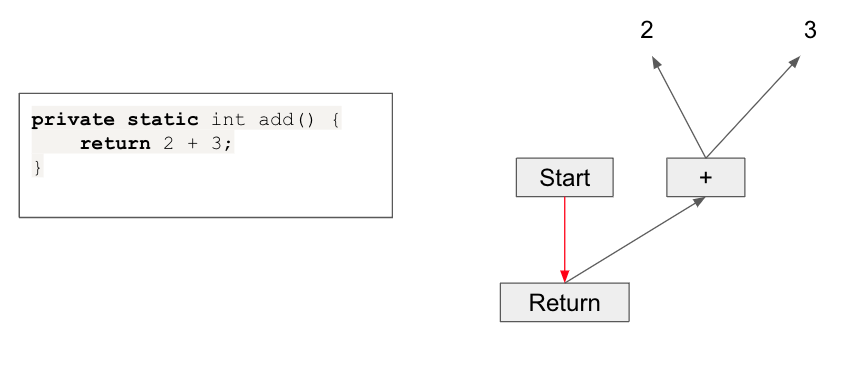
\includegraphics[width=1\textwidth]{Packages/graphir.png}
    \caption{Simple IR Graph}
    \label{figure:graphir}
\end{figure}

\autoref{figure:graphir} illustrates a simple IR graph, with control flow edges highlighted in red. The graph begins at the Start node, which connects to the Return node via a successor edge. Prior to reaching the Return node, the graph traverses upward through data flow edges to compute the expression’s value. This traversal demonstrates how control and data flows interact to process and complete the function's execution.

\subsection{Logic Programming Language Prolog}

In traditional imperative languages, a program consists of a sequence of instructions. This approach emphasizes a step-by-step procedure where each instruction modifies the state of the machine to solve a given problem. In contrast, logic programming languages, such as Prolog, operate on a fundamentally different paradigm. Instead of prescribing a sequence of operations, logic programming focuses on defining a knowledge base composed of facts and rules \cite{Bramer2013}. After that, users can query the knowledge base to search for objects and relations. 

In Prolog, facts represent objects and their relationships, while rules imply the relationship between objects given it satisfies all the conditions. Once the knowledge base is established, users can formulate queries to extract information or solve problems by leveraging the logical relationships defined in the base using the depth-first search algorithm \cite{Chowdhary2020}. There may be several ways to achieve a given goal. The system initially selects the first available option. If Prolog fails to resolve a specific subgoal, it will backtrack to explore these previously noted alternatives. This mechanism, referred to as backtracking \cite{Chowdhary2020}, enables Prolog to systematically search for different solutions by revisiting and trying alternative paths.

\begin{figure}[h]
    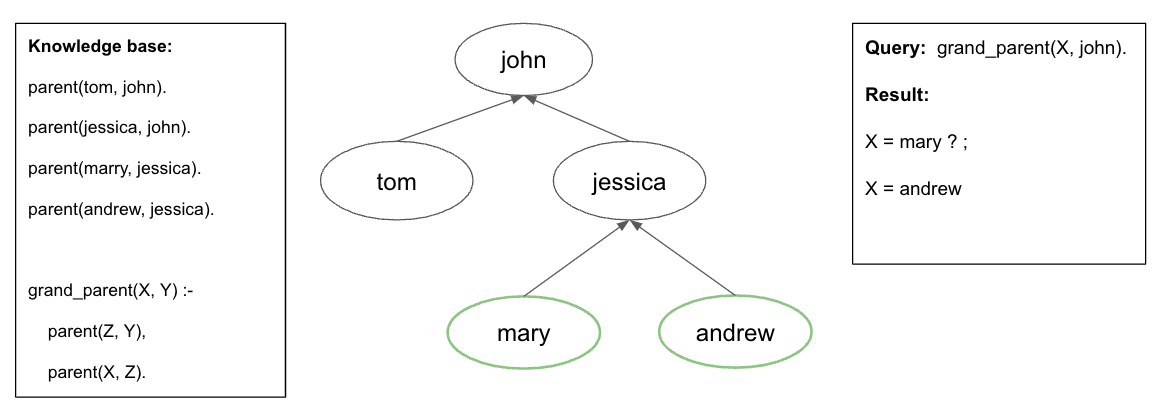
\includegraphics[width=1\textwidth]{Packages/Prolog.png}
    \caption{Example of Prolog specification}
    \label{figure:prolog}
\end{figure}

\autoref{figure:prolog}  illustrates a Prolog program. The first and final clauses are facts, specifying that nodeA is the parent of both nodeB and nodeC. In contrast, the intermediate clause represents a rule, which defines that nodeA is not the parent of nodeD. When a query is made to determine the nodes for which nodeA is a parent, Prolog executes a search from the first to the last clause, demonstrating its backtracking behavior.

\section{Literature Review}

\subsection{Advancements Through Domain-Specific Languages (DSLs)}
Declarative domain-specific languages (DSLs) have made a big impact on compiler optimization by offering targeted solutions for specific optimization tasks. For example, the Halide programming language improves image processing by separating the algorithm from its schedule, essentially the optimizations applied to the code \cite{Jonathan2018}. This separation allows for efficient and parallelized implementations with less manual effort. However, automating scheduling and keeping algorithms modular, especially as they grow in complexity, remains a challenge. Meanwhile, Spinellis created a peephole optimizer that uses a declarative DSL to specify optimizations \cite{Spinellis1999}. It turns these specifications into string regular expressions, which are then applied to the target code, allowing for adaptive and efficient refinements. Although this method has only been tested on smaller programs and specific types of optimizations so far, it shows great potential for quickly experimenting with new techniques and architectures. Elevate \cite{Hagedorn2020} is another functional language designed to let programmers define custom optimization strategies. It allows for creating composable optimizations rather than sticking to predefined APIs. Its success in case studies and practical applications highlights its ability to handle complex optimization tasks and deliver strong performance.

\subsection{Advancements Through Logic Programming Languages}
DataLog has established itself as a powerful tool in compiler implementation through its applications in complex program analysis and transformation. For instance, Lam et al. developed a framework using Datalog queries and a specialized language called PQL, which employs deductive databases and binary decision diagrams (BDDs) to tackle complex issues like pointer aliasing and heap object management in a context-sensitive manner \cite{Lam2005}. This approach has simplified the creation of sophisticated analyses and has been crucial in identifying security vulnerabilities in C and Java applications. Similarly, the Doop framework \cite{Bravenboer2009} utilizes Datalog to offer a declarative solution for points-to analysis in Java, providing impressive performance gains and scalability for precise context-sensitive analyses that were previously challenging to achieve. Furthermore, the Soufflé Datalog engine \cite{silverman2021wantanalyzeschemeprograms} introduces a new method for control-flow analysis in Scheme, making it possible to perform scalable and complex analyses of functional programming constructs, and extending the benefits of Datalog-based static analysis to Scheme-like languages. Finally, DIMPLE \cite{Benton2007}, a framework for Java bytecodes static analyses, is implemented in the Yap Prolog system. DIMPLE leverages logic programming capabilities to provide a declarative language for specifying analyses and representing Java bytecodes. The framework facilitates iterative experimentation and delivers efficient implementations that are on par with specialized tools.

\subsection{Transformation, Rewriting Techniques, and Verification}
Transformation and rewriting techniques are essential components of modern compiler optimization, enabling sophisticated processes like grammar specification, pattern matching, and program rewriting. Stratego \cite{Eelco2001} distinguishes between rewriting strategies and transformation rules, which allows for a highly flexible and controlled approach to applying optimization rules. The Stratego compiler translates these specifications into C code and leverages the ATerm library for effective term representation. It incorporates various optimizations, such as aggressive inlining and pattern merging, although it still encounters challenges related to compilation speed and support for separate compilation \cite{Eelco2001}. On the other hand, Veriopt \cite{Webb2023} offers a comprehensive framework for formally verifying optimization rules used in the GraalVM compiler. This framework employs term rewriting rules on an abstract term representation and then maps these rules to term graph transformations. Veriopt has successfully validated 45 optimization rules for GraalVM’s intermediate representation, thus advancing the reliability and effectiveness of compiler optimizations.

\subsection{Identified Research Gaps}
Despite the established effectiveness of logic programming languages like Datalog in program analysis, there is limited research on integrating these techniques within modern compiler frameworks such as GraalVM. While significant advancements have been made in transformation and rewriting techniques using domain-specific languages (DSLs) and other paradigms, there is a notable absence of comparative studies on incorporating logic programming-based optimizations into GraalVM. This gap extends to a lack of empirical evidence assessing the impact of such techniques on optimization time and efficiency. Integrating Prolog-based rules with GraalVM’s graph-based intermediate representation (IR) is particularly challenging due to insufficient research on mapping Graal IR to Prolog and ensuring that Prolog-based optimizers work effectively within the Java environment. Addressing these challenges could enhance our understanding of how to apply logic programming in modern compilers and improve compiler optimization practices by providing valuable insights into the performance and effectiveness of these techniques.
